\chapter{Recurrent Neural Networks}\label{ch:rnn}

\section{Recurrent Neural Networks}
\begin{figure}
	\begin{center}
		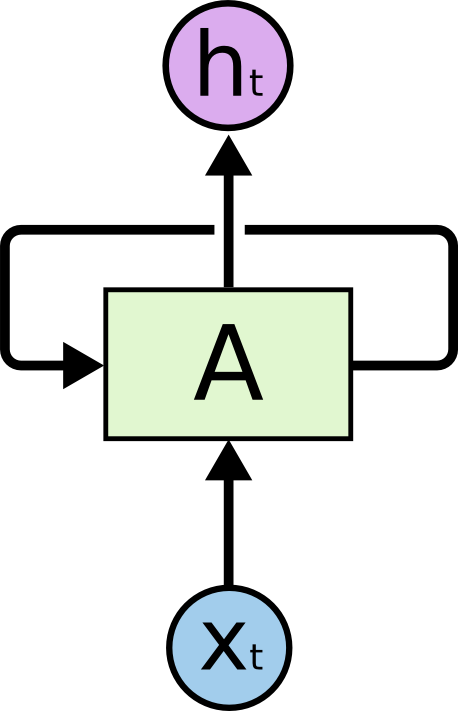
\includegraphics[scale=0.5]{rnn/rnn_rolled}
	\end{center}
	\caption{A recurrent neural network. From~\cite{RNNRolled2015}\label{fig:rnn_img}}
\end{figure}

A recurrent neural network (RNN) is a variation of artificial neural networks that continuously uses the output of its previous layer as the input of the current layer along with the input that was inputted to this iteration (see figure~\ref{fig:rnn_img}). Because of this feature, RNNs have the ability to store and keep in memory previous input values as they can be passed along through the previous iteration's output. 

\begin{figure}
	\begin{center}
		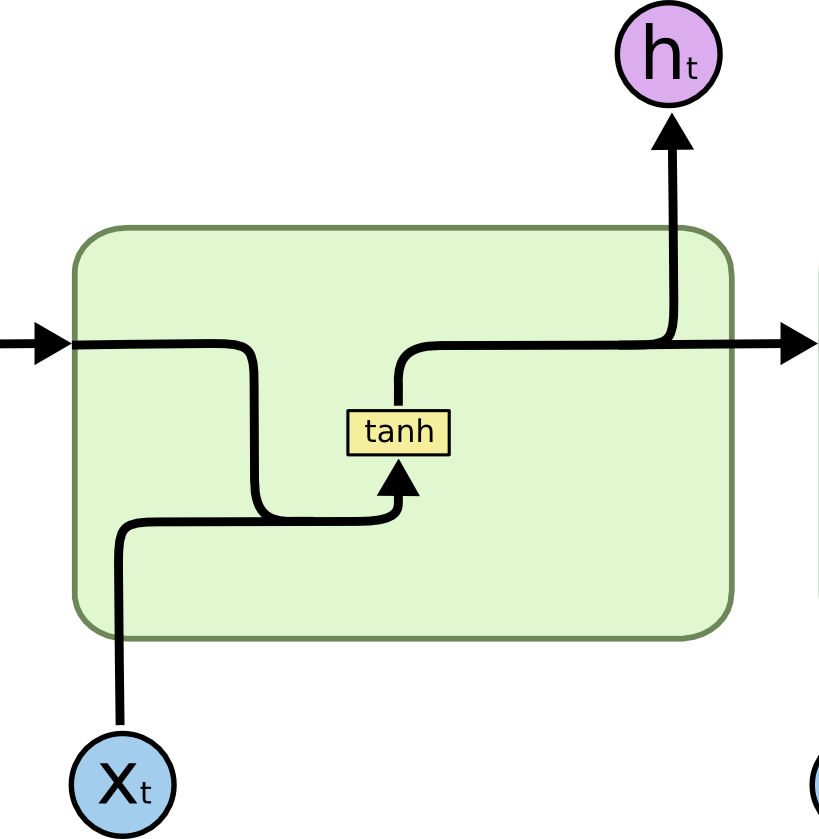
\includegraphics[scale=0.5]{rnn/rnn_cell}
	\end{center}
	\caption{A single RNN cell. From~\cite{SimpleRNN2015}\label{fig:rnn_cell}}
\end{figure}

As can be seen in figure~\ref{fig:rnn_cell}, RNNs only have a single value that acts as both the output of the cell and the data passed through to the next iteration. This hidden layer value h\(_{\text{t}}\) at time step t is calculated by the following function where h\(_{\text{t}}\) is the value of the current hidden state and output and h\(_{\text{t-1}}\) the value of the previous hidden state, \(W\) is the weight matrix for the cell's input, \(U\) is the weight matrix for the hidden value, x\(_{\text{t}}\) is the input of this cell, and \(\sigma \) is a sigmoid function used to squash its inputs into the [-1, 1] range:

$$ h_t = \sigma(Wx + Uh_\text{t-1}) $$

%cSpell:words bengio hochreiter
In theory the RNN has the ability to recall previous inputs, however in practice standard RNNs seem to be not that amazing at remembering data for long periods of time. This problem was investigated in~\cite{bengio1994learning} among others, finding problems with gradient based learning algorithms when applied to RNNs. This then prompted the development of the commonly used LSTM RNN, introduced by~\cite{hochreiter1997long}\@.

\section{LSTMs}

\begin{figure}
	\begin{center}
		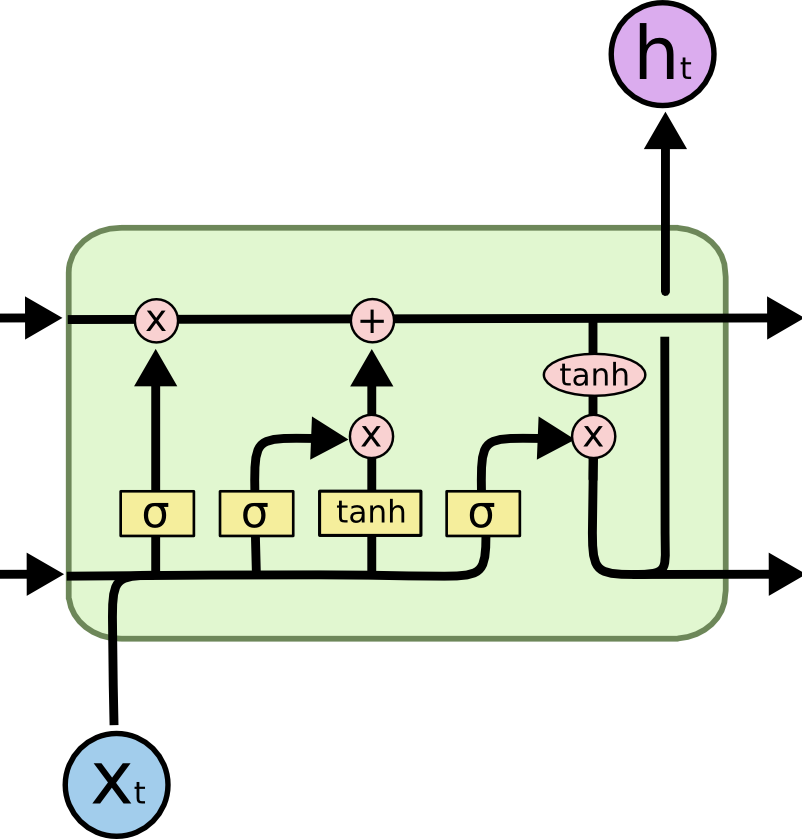
\includegraphics[scale=0.5]{rnn/lstm_cell}
	\end{center}
	\caption{A single LSTM cell. From~\cite{LSTMCell2015}\label{fig:lstm_cell}}
\end{figure}

Contrary to regular RNNs, LSTMs have an additional hidden state that is never directly outputted (see figure~\ref{fig:lstm_cell}). This additional hidden state can then be used by the network solely for remembering previous relevant data. Instead of having to share its \enquote{memory} with its output, these values are now separate. This has the advantage of the network never having to forget things, as remembering is its default state, seeing as the same state keeps going on to the next iteration.

As can be seen in the figure, there are quite a bit more parameters to this cell than a normal RNN cell. The output value and hidden value are composed of a number of different functions. First of all the network determines how much of the hidden state to forget, also called the forget gate. This is done by running both the previous iteration's output (\(c_{t-1}\)) and the forget gate vector (\(f_t\)) through a matrix multiplication. \(f_t\) can be obtained by using the following formula, where \(W\) contains the weights for the input and \(U\) contains the weights for the previous iteration's output vector, \(x_t\) refers to the input, \(h_{t-1}\) to the previous iteration's output vector and \(b\) to a set of vectors:

$$ f_t = \sigma(W_f x_t + U_f h_{t-1} + b_f) $$

The network then determines what to remember from the input values. This is commonly referred to as the input gate. This is done by running the previous forget gate's result and the input gate through a matrix addition function. The input gate (\(i_t\)) can be found by using the following formula:

$$ i_t = \sigma(W_i x_t + U_i h_{t-1} + b_i) $$

The final value of the hidden state (\(c_t\)) can then be found by using the previous two results as follows, where \(\circ \) is the Hadamard product (where each value at index \(ij\) is the product of the values at the indexes \(ij\) in the two input matrices): 

$$ c_t = f_t \circ c_{t-1} + i_t \circ \sigma(W_c x_t + U_c h_{t-1} + b_c) $$

This value is then passed on to the next iteration. Now the output gate value \(o_t\) is calculated:

$$ o_t = \sigma(W_o x_t + U_o h_{t-1} + b_o) $$

The output value \(h_t\) can then be obtained:

$$ h_t = o_t \circ \sigma(c_t) $$

\begin{figure}
	\begin{center}
		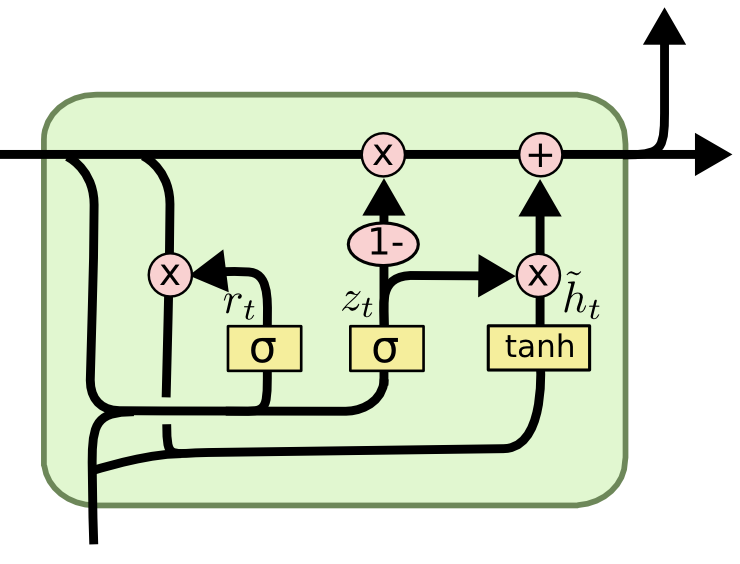
\includegraphics[scale=0.5]{rnn/gru_cell}
	\end{center}
	\caption{A single GRU variation cell. From~\cite{GRU2015}\label{fig:gru_cell}}
\end{figure}

%cSpell:words gers jozefowicz
This results in a version of an RNN that is able to remember more and is more liberal in choosing what it wants to remember and what it wants to discard. This allows them to be used a lot more effectively and has lead to the LSTM becoming the dominant RNN architecture. There have been numerous variations of the standard LSTM architecture that was just described, including but not limited to the Depth Gated RNN~\cite{yao2015depth}, which uses an additional depth gate to connect memory cells of adjacent layers, the Peephole LSTM~\cite{gers2002learning} that connects the hidden state with the gate activation functions, and the Gated Recurrent Unit (GRU)~\cite{cho2014learning} that combines the input and forget gates into a single so-called \enquote{update gate} (see figure~\ref{fig:gru_cell}). There has been some research into which architectures are the most efficient.~\cite{jozefowicz2015empirical} found that some architectures did work better than others, however seeing as this study did not include a variation of anomaly detection in its testing problems, we'll be using the standard LSTM architecture.